\section{Marco Teórico}

\subsection{Principio de Funcionamiento del Transformador Monofásico}

Un transformador monofásico ideal está compuesto por dos devanados eléctricamente aislados, arrollados sobre un núcleo ferromagnético común. Cuando se aplica una tensión alterna $v_1(t)$ al devanado primario, circula una corriente $i_1(t)$ que genera una fuerza magnetomotriz $N_1i_1(t)$. Esta fuerza establece un flujo magnético $\phi(t)$ en el núcleo, el cual, al ser variable en el tiempo, induce fuerzas electromotrices en ambos devanados según la Ley de Faraday:

\begin{equation}
v_1(t)=N_1\frac{d\phi}{dt},\qquad v_2(t)=N_2\frac{d\phi}{dt}
\end{equation}

De las expresiones anteriores se deduce la relación de transformación ideal:

\begin{equation}
\frac{V_1}{V_2}=\frac{N_1}{N_2}=a
\end{equation}

donde $a$ es la relación de transformación. En un transformador real, sin embargo, existen pérdidas en el núcleo (por histéresis y corrientes de Foucault), pérdidas Joule en los devanados, flujos de fuga y corriente de magnetización, que deben ser modelados mediante un circuito equivalente.

\subsection{Circuito Equivalente del Transformador Real}

El circuito equivalente del transformador monofásico permite representar sus propiedades eléctricas y magnéticas mediante elementos concentrados. Existen dos variantes principales: el circuito equivalente con rama en paralelo (excitación) y sus parámetros referidos al primario o al secundario.

\subsubsection{Parámetros Serie}

\begin{itemize}
	\item $R_1$, $R_2$: Resistencias de los devanados primario y secundario, que modelan las pérdidas Joule ($P_{cu}=I^2R$).
	\item $X_{f1}$, $X_{f2}$: Reactancias de fuga de los devanados primario y secundario, debidas al flujo magnético que no enlaza ambos devanados simultáneamente.
\end{itemize}

\subsubsection{Parámetros de Excitación (Rama en Paralelo)}

\begin{itemize}
	\item $R_c$: Resistencia de pérdidas en el núcleo, que representa las pérdidas activas por histéresis y corrientes de Foucault.
	\item $X_m$: Reactancia de magnetización, que modela la corriente necesaria para establecer el flujo magnético en el núcleo.
\end{itemize}

La figura 1 ilustra el circuito equivalente completo, típicamente referido al primario.

\begin{figure}[H]
	\centering
	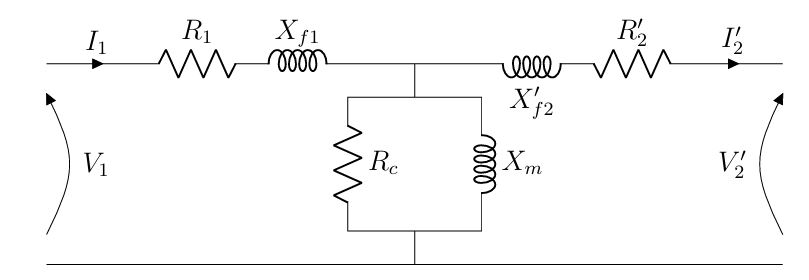
\includegraphics[width=0.85\textwidth]{imagenes/circuito primario.JPG}
	\caption{Circuito equivalente de un transformador monofásico referido al primario.}
\end{figure}

\subsection{Ensayos de Determinación de Parámetros}

\subsubsection{Medición de Resistencia de Devanados}

La resistencia óhmica de los devanados se mide por el método del voltímetro-amperímetro o mediante puente de Wheatstone o Kelvin. La norma COVENIN 3172-95 establece que la corriente de ensayo no debe exceder el $15\%$ de la corriente nominal del devanado para evitar calentamiento apreciable. El valor medido a temperatura ambiente ($T_A$) se refiere a la temperatura de operación ($T_O$) mediante:

\begin{equation}
R_T=R_m\frac{T_O+T_k}{T_A+T_k}
\end{equation}

donde $T_k=234,5\,^{\circ}\mathrm{C}$ para el cobre y $T_k=225\,^{\circ}\mathrm{C}$ para el aluminio.

\subsubsection{Medición de la Relación de Transformación}

Se aplica una tensión reducida (no menor del $20\%$ de la tensión nominal) al devanado de alta tensión y se mide la tensión inducida en el de baja tensión con dos voltímetros leídos simultáneamente. Se realizan cuatro lecturas con incrementos del $10\%$ del valor inicial y luego se repite la serie con los instrumentos intercambiados para compensar errores sistemáticos. La relación de transformación se calcula como:

\begin{equation}
a=\frac{V_{AT}}{V_{BT}}
\end{equation}

\subsubsection{Verificación de Polaridad}

La polaridad de un transformador monofásico puede ser aditiva o sustractiva. Para determinarla, se conecta el devanado de alta tensión a una fuente de CA y se unen un terminal de alta con uno de baja. Midiendo entre los terminales libres, si la lectura es superior a la tensión aplicada al primario, la polaridad es aditiva; si es inferior, es sustractiva:

\begin{equation}
E_x>E_p\qquad\text{(polaridad aditiva)}
\end{equation}

\begin{equation}
E_x<E_p\qquad\text{(polaridad sustractiva)}
\end{equation}

\subsubsection{Ensayo de Cortocircuito}

El ensayo de cortocircuito permite determinar las pérdidas en el cobre ($P_{cu}$), la impedancia de cortocircuito ($Z_{cc}$) y la tensión de cortocircuito ($V_{cc}$). Se cortocircuita el devanado de baja tensión y se aplica al de alta una tensión reducida hasta que circule entre el $75\%$ y el $100\%$ de la corriente nominal. A partir de las lecturas del vatímetro, voltímetro y amperímetro se obtienen:

\begin{equation}
P_{cc}=\text{lectura del vatímetro}
\end{equation}

\begin{equation}
Z_{cc}=\frac{V_{cc}}{I_{cc}}
\end{equation}

\begin{equation}
R_{cc}=\frac{P_{cc}}{I_{cc}^{2}}
\end{equation}

\begin{equation}
X_{cc}=\sqrt{Z_{cc}^{2}-R_{cc}^{2}}
\end{equation}

Los valores se corrigen a temperatura de operación aplicando los factores de corrección establecidos en COVENIN 3172-95.

\subsubsection{Ensayo de Vacío}

El ensayo de vacío (o de circuito abierto) determina las pérdidas en el hierro ($P_{Fe}$), la corriente de vacío ($I_0$), la resistencia de pérdidas en el núcleo ($R_c$) y la reactancia de magnetización ($X_m$). Se aplica tensión nominal al devanado de baja tensión con el de alta en circuito abierto. Las mediciones se realizan para distintos niveles de tensión: $0,5V_n$, $0,8V_n$, $1,0V_n$ y $1,1V_n$.

\begin{equation}
P_0=\text{lectura del vatímetro}
\end{equation}

\begin{equation}
R_c=\frac{V_0^2}{P_0}
\end{equation}

\begin{equation}
X_m=\frac{V_0}{\sqrt{I_0^2-(P_0/V_0)^2}}
\end{equation}

\subsection{Normas Aplicables}

\subsubsection{COVENIN 3172-95: Transformadores de Potencia -- Métodos de Ensayo}

Esta norma venezolana establece los procedimientos estandarizados para la realización de ensayos en transformadores de potencia y distribución. Define las condiciones de medición, los factores de corrección por temperatura, las tolerancias admisibles y los requisitos de seguridad para cada tipo de ensayo, incluyendo la medición de resistencia, relación de transformación, polaridad, pérdidas en vacío y pérdidas bajo carga.
